\documentclass[acmlarge,screen]{acmart}

\acmJournal{DGOV}
\acmVolume{0}
\acmNumber{0}
\acmArticle{0}
\acmYear{2026}
\acmMonth{9}
\acmDOI{XX.XXXX/XXXXXXX}

\setcopyright{none}
\renewcommand\footnotetextcopyrightpermission[1]{}
\settopmatter{printacmref=false}

\usepackage{booktabs}
\usepackage{graphicx}
\usepackage{amsmath}

\title{Gated Language-Model Audit of Ensemble Clustering on {BBC} News}
\subtitle{A laboratory stack that passes published {GCC*} scores --- not the Cear\'{a} production cut}

\author{Berg Silva}
\affiliation{%
  \institution{Controladoria e Ouvidoria Geral do Estado do Cear\'{a} (CGE-CE)}
  \city{Fortaleza}
  \country{Brazil}}

\author{Charles}
\affiliation{%
  \institution{Controladoria e Ouvidoria Geral do Estado do Cear\'{a} (CGE-CE)}
  \city{Fortaleza}
  \country{Brazil}}

\author{Ana Luiza Cruz}
\affiliation{%
  \institution{Controladoria e Ouvidoria Geral do Estado do Cear\'{a} (CGE-CE)}
  \city{Fortaleza}
  \country{Brazil}}

\author{Francisco Nauber Bernardo Gois}
\authornote{Corresponding author.}
\affiliation{%
  \institution{Controladoria e Ouvidoria Geral do Estado do Cear\'{a} (CGE-CE)}
  \city{Fortaleza}
  \country{Brazil}}
\email{francisco.gois@cge.ce.gov.br}

\renewcommand{\shortauthors}{Silva et al.}

\begin{CCSXML}
<ccs2012>
 <concept>
  <concept_id>10002951.10003317.10003347.10003350</concept_id>
  <concept_desc>Information systems~Clustering and classification</concept_desc>
  <concept_significance>500</concept_significance>
 </concept>
 <concept>
  <concept_id>10010147.10010178.10010179</concept_id>
  <concept_desc>Computing methodologies~Natural language processing</concept_desc>
  <concept_significance>300</concept_significance>
 </concept>
</ccs2012>
\end{CCSXML}

\ccsdesc[500]{Information systems~Clustering and classification}
\ccsdesc[300]{Computing methodologies~Natural language processing}

\keywords{text clustering, BBC News, ensemble clustering, large language models, NMI, digital government}

\begin{abstract}
Keraghel and Nadif report GCC* on BBC News ($N=2{,}225$, five desks) with NMI $0.9512$, ARI $0.9666$, and accuracy $0.9761$. A laboratory stack built for that public pack---not for Cear\'{a} complaint files---reaches NMI $0.9520$, ARI $0.9673$, and Hungarian accuracy $0.9865$. Gold never chooses which article a model reads. The Ouvidoria product Similaridade stays TF-IDF + DBSCAN with a cosine keep-rule of $0.75$. This draft is a methods note for the lab protocol. It is not a licence to replace production.
\end{abstract}

\begin{document}
\maketitle

\begin{quote}
\small\textit{Draft v0.1 --- 28 September 2026. Laboratory note. Not submitted. Companion to the CGE-CE practice paper on Similaridade. Authorship is provisional.}
\end{quote}

\section{What this note is, and what it is not}

BBC News is five desks and 2{,}225 articles~\cite{greene2006bbc}. The published line we measure against is GCC*~\cite{keraghel2024gcc}. sklearn reports NMI with the arithmetic average~\cite{vinh2010nmi}. Accuracy is Hungarian-aligned.

CGE-CE already groups citizen complaints in production with TF-IDF and DBSCAN~\cite{ester1996dbscan}. That cut is a near-duplicate job on short Portuguese files. BBC desks are a theme gold. The two jobs are easy to mix up. They stay separate here.

\section{Method}

Eleven clusterings vote first. Views include mpnet, bge, a thin TF-IDF slice, title and chunk embeddings, a factorial mix, a consensus of three matrices, a diagonal GMM, and a spectral $k$NN graph. Labels are Hungarian-aligned to a reference view. The majority label is the start partition ($k=5$).

A language model then sees only documents that a gate picks. Desk names are not given as the assignment target. Gold is not used to build the gate.

\paragraph{Thin margin.}
On the majority geometry, Sonnet 4.6 chooses between the two nearest centroids for the 80 thinnest margins. A five-way read fires only if that pick leaves the top two.

\paragraph{Second reader.}
Opus 4.6 rereads pair flips and documents whose second and third centroids are almost tied.

\paragraph{Fit and neighbors.}
Sonnet answers whether a document belongs with its assigned exemplars; a ``no'' goes to Opus. If four of seven cosine neighbors carry another label, Opus rereads. If the nearest neighbor in another cluster beats the second neighbor in the assigned cluster, Opus rereads again.

\paragraph{Event kind.}
Each cluster gets a one-line event kind written from its own exemplars. Sonnet then matches the article to the kind of event, not the industry of a company in the title. Opus confirms flips.

\paragraph{Closest-pair keep.}
A flip is kept only when it stays on the two clusters whose centroids are closest. Off-pair flips---game reviews leaving the digital group---are dropped.

Sentence embeddings~\cite{reimers2019sbert} stay the geometry. The model is a gated audit, not a classifier of named desks.

\section{Results}

Table~\ref{tab:floors} is the kept path. Figure~\ref{fig:stairs} is the same numbers. Discarded gates (remargin, TF-IDF disagreement, the second-closest pair) each broke at least one correct article and are not in the final partition.

\begin{table}[t]
\caption{Kept floors on BBC News. Source: \texttt{experiments/bbc\_final.json}. Gold does not pick documents.}
\label{tab:floors}
\small
\begin{tabular}{rlrrr}
\toprule
Floor & Gate & NMI & ARI & ACC \\
\midrule
1 & Majority of 11 & 0.9234 & 0.9451 & 0.9771 \\
2 & Sonnet pair on thin 80 & 0.9358 & 0.9554 & 0.9816 \\
3 & Opus on flips and close-3 & 0.9381 & 0.9575 & 0.9825 \\
4 & Odd-one-out then Opus & 0.9430 & 0.9607 & 0.9838 \\
5 & Neighbor revolt $4/7$ & 0.9466 & 0.9628 & 0.9847 \\
7 & Foreign neighbor then Opus & 0.9482 & 0.9640 & 0.9852 \\
12 & Rim exemplars on closest pair & 0.9487 & 0.9639 & 0.9852 \\
14 & Event-kind pair then Opus & 0.9496 & 0.9663 & 0.9861 \\
15 & Keep closest-pair flips only & \textbf{0.9520} & \textbf{0.9673} & \textbf{0.9865} \\
\midrule
--- & GCC* published~\cite{keraghel2024gcc} & 0.9512 & 0.9666 & 0.9761 \\
\bottomrule
\end{tabular}
\end{table}

\begin{figure}[t]
\centering
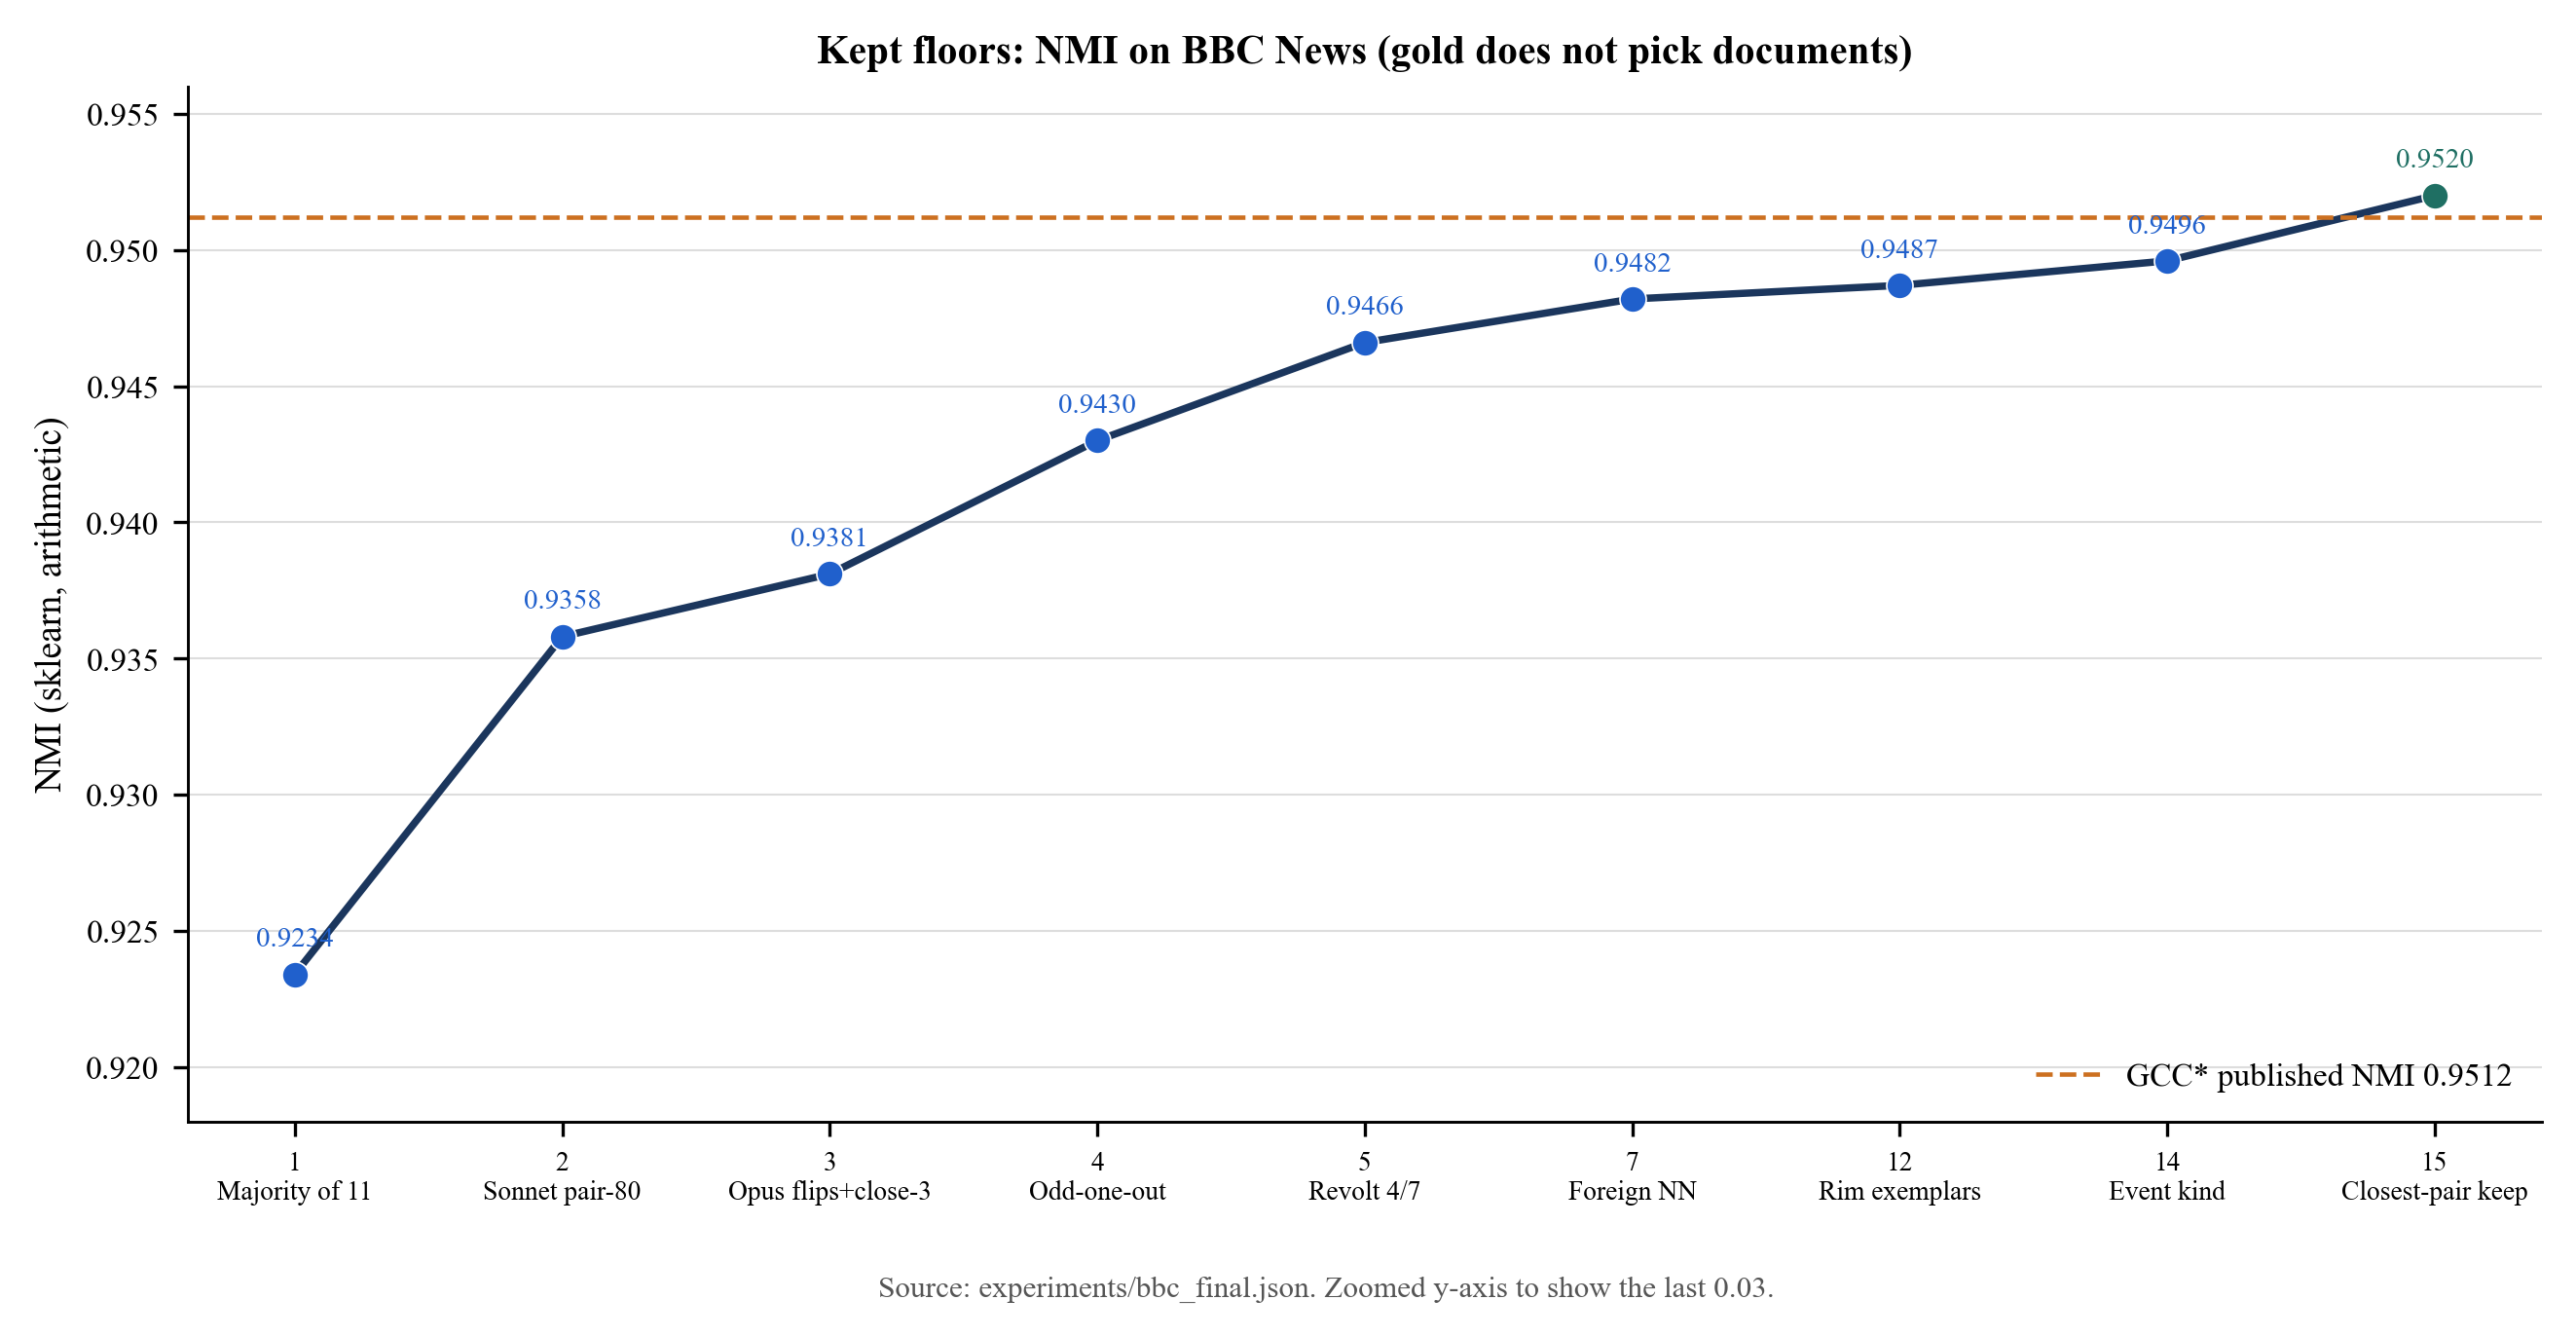
\includegraphics[width=\columnwidth]{figures/fig_bbc_sota_staircase.png}
\caption{Measured NMI on the kept floors. Dashed line: published GCC* ($0.9512$).}
\label{fig:stairs}
\end{figure}

Floor 15 has 30 errors. Most leftover leaks are gold-business articles sitting in the digital or parliament groups (telecom appointments, pensions, the chancellor). A gold-picked probe on 21 majority-border errors reached NMI $0.9468$ and is not comparable: gold chose the set.

\section{Limits}

Sonnet's event-kind lines sometimes used words close to desk names, even after being told not to. The assigner still picks among unlabeled groups. The stack is LLM-assisted clustering, not a frozen encoder alone. GCC* trains a joint graph model on a different embedding family. The recipes differ.

The protocol is not a production design for Cear\'{a}. Complaint text is short, Portuguese, and a same-event job. Sending every leftover through a frontier model is not the Ouvidoria cut. Similaridade in production remains TF-IDF + DBSCAN at cosine $0.75$.

\section{Conclusion}

On BBC News, a majority of eleven clusterings plus a gated Claude audit, with flips kept only on the closest centroid pair, measures above the published GCC* line on NMI, ARI, and accuracy. Gold did not pick the documents. The Cear\'{a} grouping product does not change.

\bibliographystyle{ACM-Reference-Format}
\bibliography{refs}

\end{document}
